\section{Introduction}

%% from the swarm vision to the necessity of selection
Increasingly, objects in our built environment are equipped with computation and communication, making them potential targets for user interaction. Such interactions might be {\em explicit} -- controlling smart appliances such as intelligent lighting, AV equipment, or HVAC systems; or {\em implicit} -- tracking the user's attention to gauge interest e.g., for targeted-advertisement or context-aware computing \bjoern{second part needs to be stronger}. Both uses rely on {\em selection} information by which a system keeps track of the user's {\em locus of attention}~\cite{raskin} in the world.

%% previous approaches are limited
Past research has introduced techniques of augmenting hand-held mobile devices with accessories like laser pointers to enable direct aiming at target devices in space~\cite{beigl_point_1999,patel_2-way_2003}. While promising, some drawbacks of using handheld devices are that the device first has to be retrieved (e.g., from a pocket) and consciously aimed (which also limits use to explicit scenarios); that the user's hands are required to be free for operation (one to hold the device, one to operate the touch screen); and that the user's visual attention is now split between looking down at a screen and out at targets in the world. 

%% introducing head-worn computing and head orientation
Emerging head-worn computing devices have the potential to overcome some of these limitations: because they are worn, they do not require retrieval; they may enable hands-free or uni-manual interactions; and they offer near-eye or see-through displays to overlay information. Also such computing devices are well aligned with the user's line of sight, which is a strong indication of the user's interaction targets \ben{citation needed here}.

%% head orientation limit
Though natural, head orientation is an imprecise indicator of the user's locus of attention: it contains the general direction, but not the particular point of focus. 
% should we argue gaze tracking doesn't help much but only increases the complexity?
Therefore, it requires area selection \bjoern{reference} combined with disambiguation techniques.

%% the inaccuracy of head orientation
In this paper, we investigate how to leverage head-orientation for target selection in physical spaces. We propose a simple low-cost solution that can be readily implemented with small hardware changes to emerging wearable devices. Specifically, we augment Google Glass\footnote{\url{http://www.google.com/glass/start/}} with custom hardware for this purpose. We use infrared (IR) communication between Glass and target appliances to capture the user's head orientation. Because IR signal usually covers a cone shape of area (a diameter of 60-120cm and distance up to 6m), it's suitable for the area selection modality. To achieve the disambiguation when multiple targets have received IR signals, we propose three different ways of disambiguation. First, the targets compare the IR signal intensity and we propose some intuitive heuristic to infer the user's intention in disambiguation. Second, we incorporate the sensors on Google Glass to track the user's head movement and combine this with IR intensity changes. Last but not least, we always leave the option of manually changing the current targets to the user such but limit the scope of potential targets to the ones that have received IR signals.
%% three ways

While prior work has tended to focus on proofs-of-concept for head-orientation based interaction, we also contribute empirical data on the system performance, usability, and user experience of head-orientation targeting and device control. We first report measurements of range and beam characteristics of our controller. We then conduct a study with $14$ participants that compares acquisition times for physical targets in a room for our technique and an alternative list selection interface. We find that target acquisition through head orientation is preferred by users and is faster than list selection, given the constraints of linear input using a head-worn touch controller. 
We then quantify the additional benefit of using IR-intensity disambiguation \bjoern{and find XYZ.}. \bjoern{Say something about the inferred map if we get around to it}.

Such head orientation-based selection enables a wide range of context-aware applications. Examples include smart home remote control, break reminder monitor starer, museum attention tracking, indoor positioning, etc. In Figure\,\ref{fig:teaser}, it's a demonstration of the ``universal remote control'' scenario. The user can easily select the smart appliances by simply looking at it's general direction and confirm such selection with either voice command or by tapping the Glass input pad. Then an appliance-specific control UI will be shown on the head-mounted display. For this application, we have asked 14 participants to try the system and we report the qualitative results from them performing home automation tasks.

\begin{figure}[t]
\centering
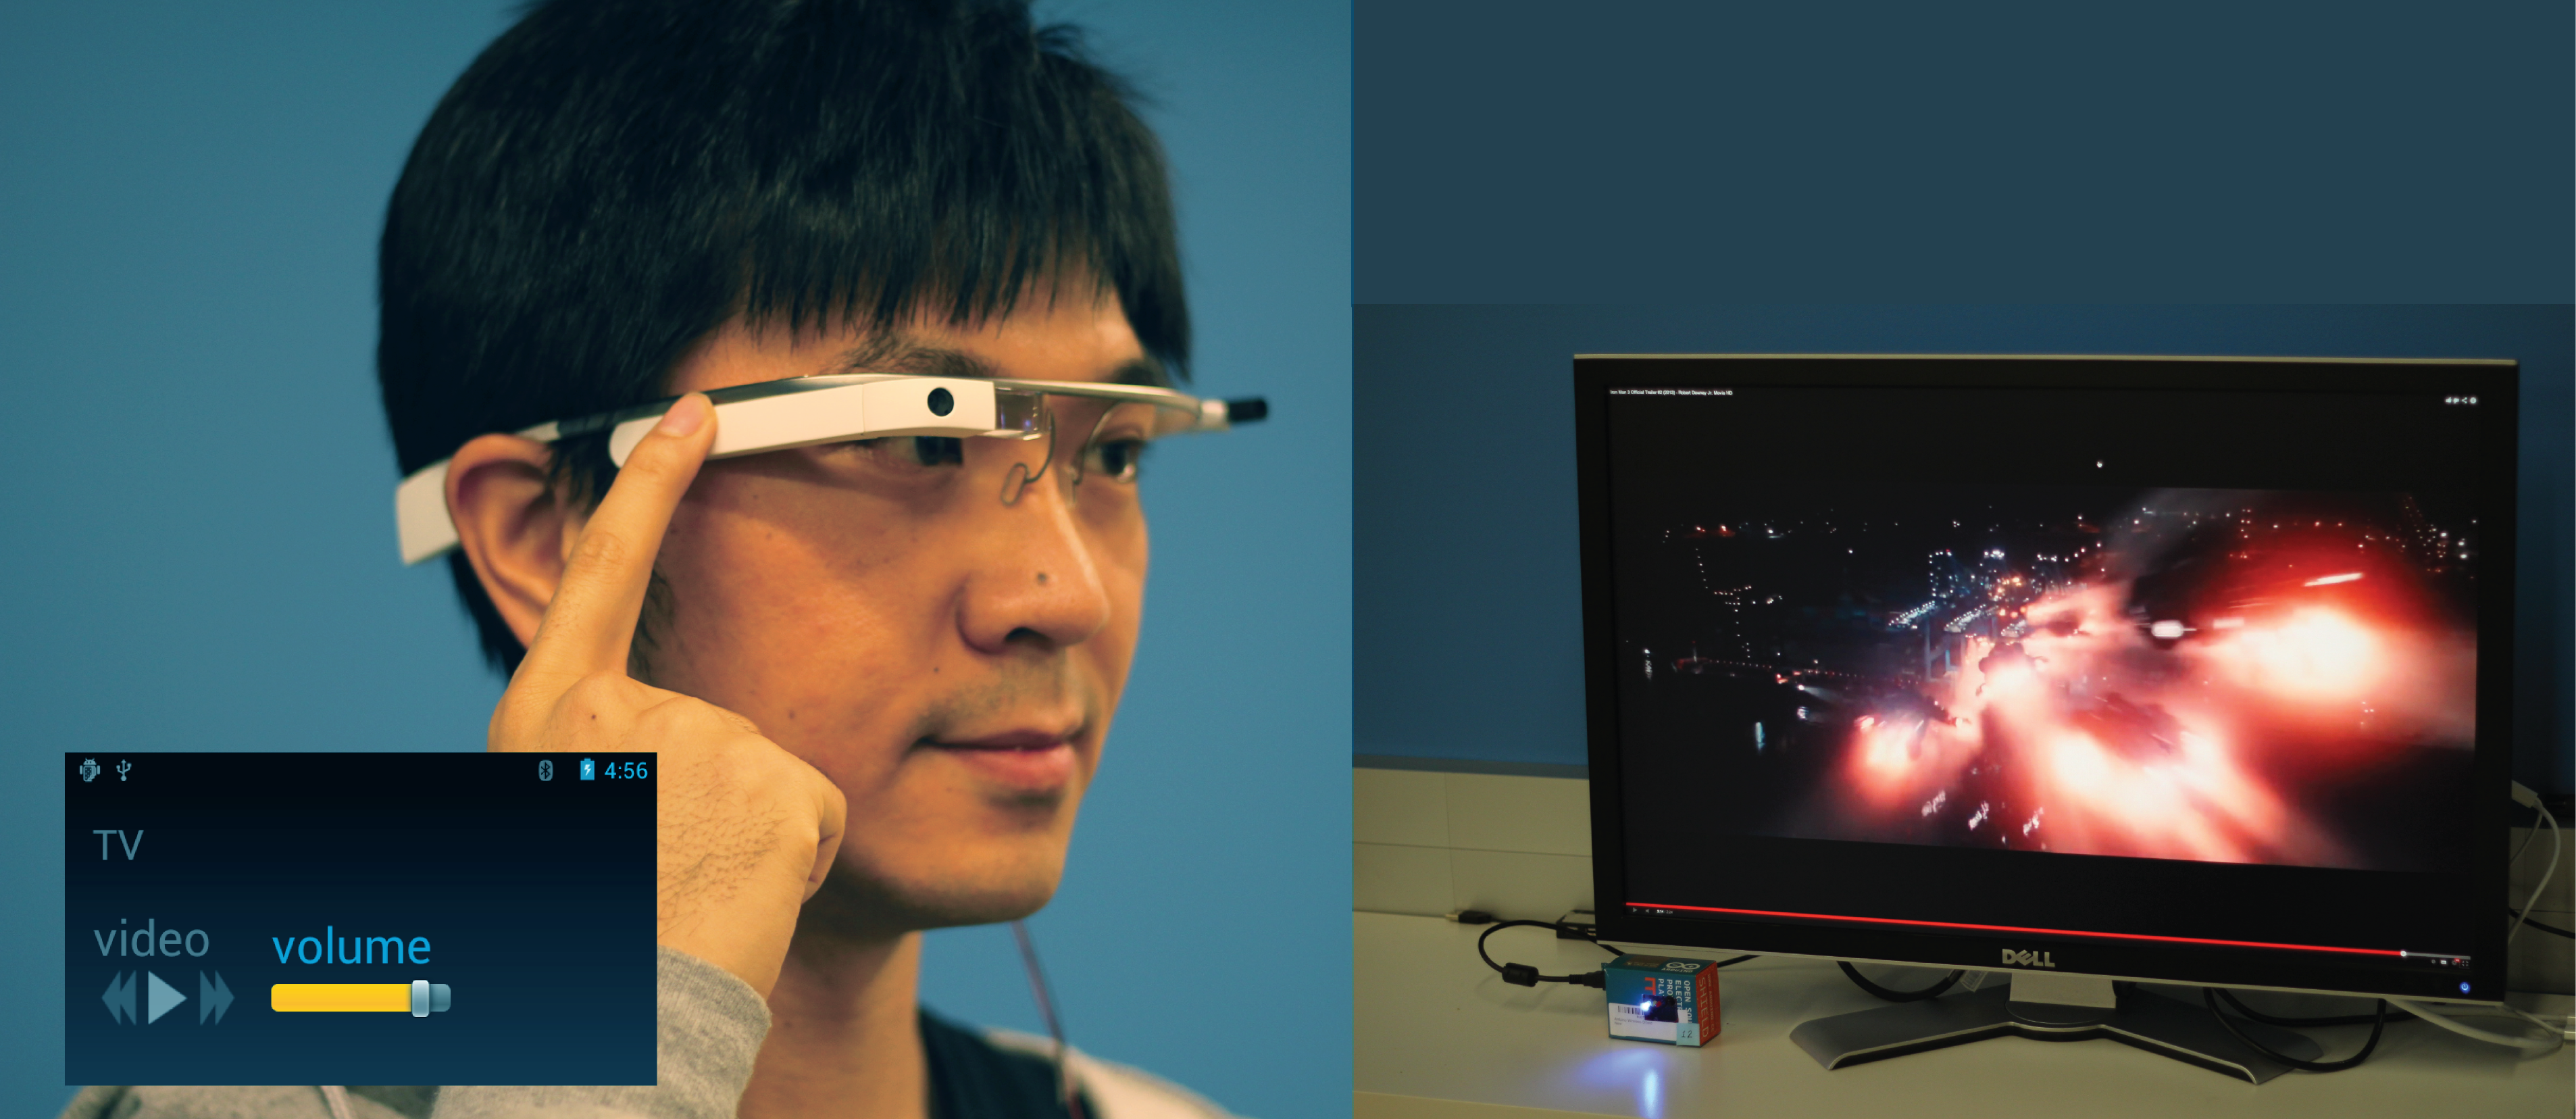
\includegraphics[width=1.0\columnwidth]{figures/teaser.jpg}
\caption{Using an augmented head-worn device (1), users can control smart home appliances (2) with head orientation targeting. A near-eye display then shows an appliance control UI (3), which users navigate through multitouch gestures.}
\label{fig:teaser}
\end{figure}

%% Contribution
In this paper, by presenting our work on head orientation-based beam cursor,  we make the following contributions:
\begin{itemize}
\item We design and implement a low-cost, easy-to-use head orientation system that enables interaction with physical environment.
\item To solve the inherent inaccuracy of head orientation, we have proposed three different ways to achieve disambiguation and we evaluate them based on real-world user study.
\item We also demonstrate that several useful applications can be easily built with the head orientation system.
\end{itemize}

\ben{Having problem fixing the reference}.
In the remainder of this paper, we will first describe the related works in physical selection and targeting. Given that we focus our scope on head orientation, in Section~\ref{sec:background} we will briefly review human's neck ergonomics as the background for head orientation. In Section~\ref{sec:syst-design-prot}, we then present our system designed for the study of head orientation based selection. The prototype is also what we have used for building the example applications. The disambiguation techniques are discussed in Section~\ref{sec:disamb-techn}, which is followed by the study and evaluation in Section~\ref{sec:evaluation}. To further show the usefulness of having such head orientation-based selection, we describe the enabled applications in Section~\ref{sec:applications}, with detailed implementation about the ``universal remote control'' application. The discussion and conclusion are in Section~\ref{sec:discussion} and Section~\ref{sec:conclusion} respectively. 

%%% Local Variables: 
%%% mode: latex
%%% TeX-master: "uist14"
%%% End: 
